% shared-layout-id: f507f74e420943715f784f06f32045d0248628be259e1505f05383c11f98d057
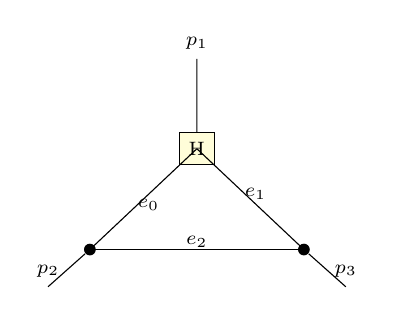
\begin{tikzpicture}[scale=.65,every node/.style={font=\scriptsize}]
\node[rectangle,draw,fill=yellow!15] (v0) at (3.27272727,3.15151515) {H};
\node[circle,fill,inner sep=1.5pt] (v1) at (1.18181818,1.18181818) {};
\node[circle,fill,inner sep=1.5pt] (v2) at (5.36363636,1.18181818) {};
\draw[black] (3.27272727,3.15151515) .. controls (2.57575758,2.49494949) and (1.87878788,1.83838384) .. (1.18181818,1.18181818);
\node at (2.32700999,2.06079173) {$e_{0}$};
\draw[black] (3.27272727,3.15151515) .. controls (3.96969697,2.49494949) and (4.66666667,1.83838384) .. (5.36363636,1.18181818);
\node at (4.41791908,2.27254161) {$e_{1}$};
\draw[black] (1.18181818,1.18181818) .. controls (2.57575758,1.18181818) and (3.96969697,1.18181818) .. (5.36363636,1.18181818);
\node at (3.27272727,1.32727273) {$e_{2}$};
\draw (v0) -- (3.27272727,4.90909091) node[above] {$p_{1}$};
\draw (v1) -- (0.36363636,0.45454545) node[above] {$p_{2}$};
\draw (v2) -- (6.18181818,0.45454545) node[above] {$p_{3}$};
\end{tikzpicture}